\section{Linear Functions}
\label{sec:linear}

% Do some regression.
% First differences.

\subsection{Linear Function Basics}

In Section \ref{ssec:cost}, we had the example of a screen printing shop that charges \$50 to cover the overhead costs of setting the screen to make T-shirts and \$5 per shirt for the shirts themselves. Using descriptive variables, we chose $n$ for the number of T-shirts and $C$ for the cost in dollars as a function of the number of shirts: $C(n)$.

We know that $C(0)$ = 50, since the overhead, or fixed, costs are charged regardless of the number of T-shirts made. Since \$5 is added for each T-shirt ordered, then $C(1) = \$50 + \$5 = \$55$, $C(2) = \$55 + \$5 = \$60$, and so on.

If $n$ T-shirts are ordered, then

$$C(n) = \$50 + \left(\frac{\$5}{\mbox{T-shirt}}\right)(n \mbox{ T-shirts}) = 50 + 5n \mbox{ dollars} \enspace .$$
Notice how the units (or dimensions) make sense in this equation. Each term has units of dollars, after cancelling the unit of ``T-shirt" in the second term.

Notice this equation consisted of two quantities. The first is the fixed \$50 charge which does not change based on the value of the input. When the no T-shirts are ordered, the cost is \$50, giving the point
$(0, 50)$ on the graph of the function. This is the {\bf vertical}\index{Intercept!vertical} or {$y$-intercept}\index{Intercept!$y$}. The second is the \$5 per T-shirt, which is a \textbf{rate of change}\index{Rate of change}. In $C(n)$, this rate of change is multiplied by the input value. It is important here to note that in this equation, the rate of change is {\bf constant}; over any interval, the rate of change is the same.

Looking at $C(n)$ as a table, we can also see the cost changes by \$5 for each additional T-shirt.

\begin{longtable}[]{@{}lrrrr@{}}
\toprule
$n$ & 0 & 1 & 2 & 3\tabularnewline
\midrule
$C(n)$ & 50 & 55 & 60 & 65\tabularnewline
\bottomrule
\end{longtable}

 (Even though we cannot order a fractional number of T-shirts, we still graph $y=C(n)$ on all $n\ge 0$.)

The graph is increasing in a straight line from left to right because for each T-shirt, the cost goes up by \$5; this rate remains consistent.

In this example, you have seen the T-shirt cost modeled in words, an equation, a table, and as a graph. Whenever possible, ensure that you can link these four representations together to continually build your skills. It is important to note that you will not always be able to find all four representations for a problem and so being able to work with all four forms is very important.

The function $C(n)$ is an example of a {\bf linear function}\index{Function!linear}. This name comes from the fact that a graph of a linear function is a line.


\begin{definition}
A \textbf{linear function} is a function whose graph produces a line. Linear functions can always be written in the form
$$f(x) = mx +b \enspace ,$$
where:\\
$b$ is the initial or starting value of the function (when the input, $x = 0$), and\\
$m$ is the constant rate of change of the function.

This form of the line is called the {\bf slope-intercept form}\index{Slope-intercept form}.
\end{definition}

Many people like to write linear functions in the form $y=mx + b$ because it corresponds to the way we tend to speak: ``The output starts at $b$ and increases at a rate of $m$.''

\paragraph{Slope and Increasing/Decreasing}

The constant rate of change of a linear function, $m$, is also called the \textbf{slope}\index{Slope} of the function. The slope determines if the function is an increasing function or a decreasing function.\\
$f(x) = mx + b$ is an \textbf{increasing}\index{Increasing} function if $m>0$.\\
$f(x) = mx + b$ is a \textbf{decreasing}\index{Decreasing} function if $m<0$.

If $m=0$, then the rate of change of $f(x) = mx+b$ is zero, and $f(x) = 0\cdot x+b = b$, so its graph is just the horizontal line passing through the point $(0, b)$, neither increasing nor decreasing.

The concepts of slope and rate of change are major component of calculus. It is crucial to understand each facet of these two concpets that we will discuss in this section since these conepts will be generalized from linear functions to a wide array of functions in Chapter \ref{ch:derivatives}.

\begin{example}
Marcus currently owns 200 songs in his iTunes collection. Every month, he adds 15 new songs. Write a formula for the number of songs, $N$, in his iTunes collection as a function of the number of months, $m$. How many songs will he own in a year?

\solution The initial value for this function is 200, since he currently owns 200 songs, $N(0)=200$ songs. The number of songs increases by 15 songs per month, so the rate of change is 15 songs per month. With this information, we can write the formula:
$$N(m) = 200 \mbox{ songs} + \left(\frac{15\mbox{ songs}}{\mbox{month}}\right)(m \mbox{ months}) = 200 + 15m \mbox{ songs} \enspace .$$

With this formula we can predict how many songs he will have in 1 year (12 months):
$$N(12) = 200 + 15\cdot 12\mbox{ songs}  = 200 + 180 = 380 \mbox{ songs}  \enspace .$$
Marcus will have 380 songs in a year.
\end{example}


\paragraph{Calculating Rate of Change}

Given two values for the input, $x_1$ and $x_2$, and two corresponding values for the output, $y_1$ and $y_2$, or a set of points, $(x_1, y_1)$ and $(x_2, y_2)$, we can find a linear function that contains both points. First we calculate the rate of change, $m$, of the function.

$$\mbox{slope}=\frac{\mbox{rise}}{\mbox{run}}=\frac{\mbox{change in } y}{\mbox{change in } x} \Rightarrow m = \frac{y_2-y_1}{x_2-x_1}$$

It is also customary to write $\Delta v$ for a change (or difference) in the variable $v$. We read this ``delta $v$"\index{Delta ($\Delta$)}. With this notation, we can write
$$m=\frac{\Delta y }{\Delta x} = \frac{y_2-y_1}{x_2-x_1}\enspace .$$

Note in function notation, $y_1 = f(x_1)$ and $y_2 = f(x_2)$, so we could equivalently write
$$m=\frac{f(x_2)-f(x_1)}{x_2-x_1}\enspace .$$

Once we have computed $m$, we can use either of the given points to find $b$ using algebra.
\begin{note}
Note: It is a waste of your time to make a special effort to memorize the following formula. This is a concept to understand.
\end{note}
\begin{align*}
y_1 &=& mx_1 + b \\
b &=& y_1 - mx_1
\end{align*}

\begin{example}
The population of a city increased from 23,400 to 27,800 between 2002 and 2006. Find the rate of change of the population during this time span.

\solution The rate of change will relate the change in population to the change in time. The population increased by people over the four-year time interval. To find the rate of change, the number of people per year the population changed by:
$$m = \frac{27800-23400 \mbox people}{2006 - 2002 \mbox{ years}} = \frac{4400\mbox{ people}}{4\mbox{ years}} = 1100 \mbox{ people per year} \enspace .$$
\end{example}
Notice that we knew the population was increasing, so we expected $m>0$. This is a quick way to check if the solution is reasonable.

\begin{example}
The pressure, $P$, in pounds per square inch (psi) on a diver depends upon their depth below the water surface, $d$, in feet, following the equation . Interpret the components of this function.

\solution The rate of change, or slope, 0.434 would have units . This tells us the pressure on the diver increases by 0.434 PSI for each foot their depth increases.

The initial value, 14.696, will have the same units as the output, so this tells us that at a depth of 0 feet, the pressure on the diver will be 14.696 psi.
\end{example}

We can now find the rate of change given two input-output pairs, and can
write an equation for a linear function once we have the rate of change
and initial value. If we have two input-output pairs and they do not
include the initial value of the function, then we will have to solve
for it.

\begin{example}

\includegraphics[width=2.22917in,height=2.05556in]{media/image35.png}Write
an equation for the linear function graphed to the right.

Looking at the graph, we might notice that it passes through the points
(0, 7) and (4, 4). From the first value, we know the initial value of
the function is $b = 7$, so in this case we will only need to
calculate the rate of change:

This allows us to write the equation:


\end{example}

\begin{example}
If is a linear function, , and , find an equation for the function.

In example 3, we computed the rate of change to be . In this case, we do
not know the initial value, so we will have to solve for it. Using the
rate of change, we know the equation will have the form. Since we know
the value of the function when $x = 3$, we can evaluate the
function at 3.

Since we know that, we can substitute on the left side

This leaves us with an equation we can solve for the initial value

Combining this with the value for the rate of change, we can now write a
formula for this function:

\end{example}
\begin{example}

Working as an insurance salesperson, Ilya earns a base salary and a
commission on each new policy, so Ilya's weekly income, $I$,
depends on the number of new policies, $n$, he sells during the
week. Last week he sold 3 new policies, and earned \$760 for the week.
The week before, he sold 5 new policies, and earned \$920. Find an
equation for $I(n)$, and interpret the meaning of the components of
the equation.

The given information gives us two input-output pairs: (3,760) and
(5,920). We start by finding the rate of change.

Keeping track of units can help us interpret this quantity. Income
increased by \$160 when the number of policies increased by 2, so the
rate of change is \$80 per policy; Ilya earns a commission of \$80 for
each policy sold during the week.

We can then solve for the initial value

then when $n = 3$, , giving

this allows us to solve for $b$

This value is the starting value for the function. This is Ilya's income
when $n = 0$, which means no new policies are sold. We can
interpret this as Ilya's base salary for the week, which does not depend
upon the number of policies sold.

Writing the final equation:

Our final interpretation is: Ilya's base salary is \$520 per week and he
earns an additional \$80 commission for each policy sold each week.
\end{example}

Flashback

Looking at Example 7:\\
Determine the independent and dependent variables.\\
What is a reasonable domain and range?\\
Is this function one-to-one?

Example 8

Given the table below write a linear equation that represents the table
values

We can see from the table that the initial value of rats is 1000 so in
the linear format

, $b = 1000$.

Rather than solving for $m$, we can notice from the table that the
population goes up by 80 for every 2 weeks that pass. This rate is
consistent from week 0, to week 2, 4, and 6. The rate of change is 80
rats per 2 weeks. This can be simplified to 40 rats per week and we can
write

as

If you didn't notice this from the table you could still solve for the
slope using any two points from the table. For example, using (2, 1080)
and (6, 1240),

rats per week
\subsection{Graphs of Linear Functions}
%\label{section-2.2-graphs-of-linear-functions}

When we are working with a new function, it is useful to know as much as
we can about the function: its graph, where the function is zero, and
any other special behaviors of the function. We will begin this
exploration of linear functions with a look at graphs.

When graphing a linear function, there are three basic ways to graph it:

\begin{enumerate}
\def\labelenumi{\arabic{enumi})}
\item
  By plotting points (at least 2) and drawing a line through the points
\item
  Using the initial value (output when $x = 0$) and rate of change
  (slope)
\item
  Using transformations of the identity function
\end{enumerate}

Example 1

Graph by plotting points

In general, we evaluate the function at two or more inputs to find at
least two points on the graph. Usually it is best to pick input values
that will ``work nicely'' in the equation. In this equation, multiples
of 3 will work nicely due to the in the equation, and of course using
$x = 0$ to get the vertical intercept. Evaluating $f(x)$ at
$x = 0, 3$, and $6$:

\includegraphics[width=2.64861in,height=2.26319in]{media/image93.png}

These evaluations tell us that the points (0,5), (3,3), and (6,1) lie on
the graph of the line. Plotting these points and drawing a line through
them gives us the graph.

When using the initial value and rate of change to graph, we need to
consider the graphical interpretation of these values. Remember the
initial value of the function is the output when the input is zero, so
in the equation , the graph includes the point $(0, b)$. On the
graph, this is the vertical intercept -- the point where the graph
crosses the vertical axis.

For the rate of change, it is helpful to recall that we calculated this
value as

\includegraphics[width=3.00000in,height=2.17986in]{media/image97.png}From
a graph of a line, this tells us that if we divide the vertical
difference, or rise, of the function outputs by the horizontal
difference, or run, of the inputs, we will obtain the rate of change,
also called slope of the line.

Notice that this ratio is the same regardless of which two points we
use.

Graphical Interpretation of a Linear Equation

Graphically, in the equation,

$b$ is the \textbf{vertical intercept} of the graph and tells us we
can start our graph at $(0, b)$

$m$ is the \textbf{slope of the line} and tells us how far to rise
\& run to get to the next point

Once we have at least 2 points, we can extend the graph of the line to
the left and right.

Example 2

Graph using the vertical intercept and slope.

The vertical intercept of the function is (0, 5), giving us a point on
the graph of the line.

\includegraphics[width=2.90347in,height=2.34444in]{media/image99.png}The
slope is . This tells us that for every 3 units the graph ``runs'' in
the horizontal, the vertical ``rise'' decreases by 2 units.

In graphing, we can use this by first plotting our vertical intercept on
the graph, then using the slope to find a second point. From the initial
value (0, 5) the slope tells us that if we move to the right 3, we will
move down 2, moving us to the point (3, 3). We can continue this again
to find a third point at (6, 1). Finally, extend the line to the left
and right, containing these points.

Try it Now

1. Consider that the slope could also be written as . Using , find
another point on the graph that has a negative $x$ value.

Another option for graphing is to use transformations of the identity
function.

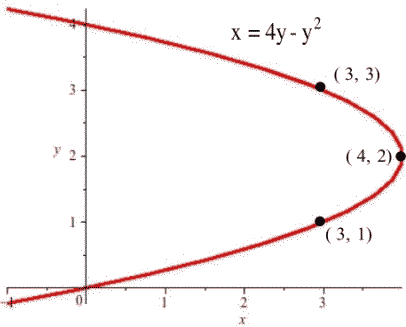
\includegraphics[width=3.70000in,height=3.76809in]{media/image103.png}

In the equation, the $m$ is acting as the vertical stretch of the
identity function. When $m$ is negative, there is also a vertical
reflection of the graph. Looking at some examples:

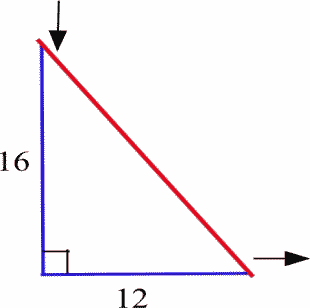
\includegraphics[width=3.70000in,height=3.69514in]{media/image105.png}

In, the $b$ acts as the vertical shift, moving the graph up and
down without affecting the slope of the line. Some examples:

Using Vertical Stretches or Compressions along with Vertical Shifts is
another way to look at identifying different types of linear functions.
Although this may not be the easiest way for you to graph this type of
function, make sure you practice each method.

Example 3

Graph using transformations.

The equation is the graph of the identity function vertically compressed
by ½ and vertically shifted down 3.

Vertical compression combined with Vertical shift

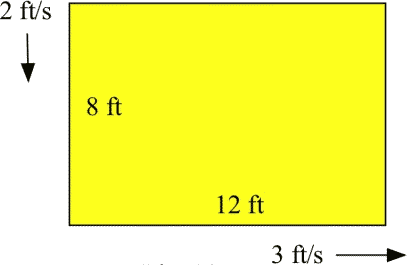
\includegraphics[width=2.43750in,height=1.75694in]{media/image108.png}
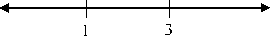
\includegraphics[width=2.37986in,height=1.70764in]{media/image109.png}

Notice how this nicely compares to the other method where the vertical
intercept is found at (0, -3) and to get to another point we rise (go up
vertically) by 1 unit and run (go horizontally) by 2 units to get to the
next point (2, -2), and the next one (4, -1). In these three points (0,
-3), (2, -2), and (4, -1), the output values change by +1, and the
$x$ values change by +2, corresponding with the slope $m = \frac{1}{2}$.

Example 4

Match each equation with one of the lines in the graph below

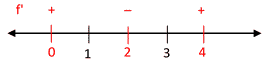
\includegraphics[width=3.09722in,height=2.33611in]{media/image110.png}

Only one graph has a vertical intercept of -3, so we can immediately
match that graph with $g(x)$.

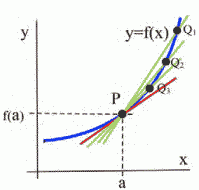
\includegraphics[width=3.05069in,height=2.28264in]{media/image112.png}For
the three graphs with a vertical intercept at 3, only one has a negative
slope, so we can match that line with $h(x)$. Of the other two, the
steeper line would have a larger slope, so we can match that graph with
equation $f(x)$, and the flatter line with the equation
$j(x)$.

In addition to understanding the basic behavior of a linear function
(increasing or decreasing, recognizing the slope and vertical
intercept), it is often helpful to know the horizontal intercept of the
function -- where it crosses the horizontal axis.

Finding Horizontal Intercepts

The \textbf{horizontal intercept} of the function is where the graph
crosses the horizontal axis. If a function has a horizontal intercept,
you can always find it by solving\\
$f(x) = 0$.

Example 5

Find the horizontal intercept of

Setting the function equal to zero to find what input will put us on the
horizontal axis,

The graph crosses the horizontal axis at (6,0)

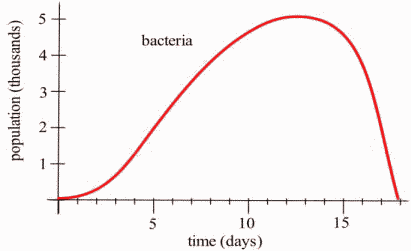
\includegraphics[width=1.85000in,height=1.83346in]{media/image114.png}There
are two special cases of lines: a horizontal line and a vertical line.
In a horizontal line like the one graphed to the right, notice that
between any two points, the change in the outputs is 0. In the slope
equation, the numerator will be 0, resulting in a slope of 0. Using a
slope of 0 in the , the equation simplifies to .

Notice a horizontal line has a vertical intercept, but no horizontal
intercept (unless it's the line $f(x) = 0$).

\includegraphics[width=1.84722in,height=1.85556in]{media/image117.png}

In the case of a vertical line, notice that between any two points, the
change in the inputs is zero. In the slope equation, the denominator
will be zero, and you may recall that we cannot divide by the zero; the
slope of a vertical line is undefined. You might also notice that a
vertical line is not a function. To write the equation of vertical line,
we simply write input=value, like.

Notice a vertical line has a horizontal intercept, but no vertical
intercept (unless it's the line $x = 0$).

Horizontal and Vertical Lines

\textbf{Horizontal lines} have equations of the form

\textbf{Vertical lines} have equations of the form $x = a$

Example 6

Write an equation for the horizontal line graphed above.

This line would have equation

Example 7

Write an equation for the vertical line graphed above.

This line would have equation

Try it Now

2. Describe the function in terms of transformations of the identity
function and find its horizontal intercept.

\textbf{Parallel and Perpendicular Lines}

When two lines are graphed together, the lines will be \textbf{parallel}
if they are increasing at the same rate -- if the rates of change are
the same. In this case, the graphs will never cross (unless they're the
same line).

Parallel Lines

Two lines are \textbf{parallel} if the slopes are equal (or, if both
lines are vertical).

In other words, given two linear equations and , the lines will be
parallel if .

Example 8

Find a line parallel to that passes through the point (3, 0)

We know the line we're looking for will have the same slope as the given
line, $m = 3$. Using this and the given point, we can solve for the
new line's vertical intercept:

then at (3, 0),

The line we're looking for is

If two lines are not parallel, one other interesting possibility is that
the lines are perpendicular, which means the lines form a right angle
(90 degree angle -- a square corner) where they meet. In this case, the
slopes when multiplied together will equal -1. Solving for one slope
leads us to the definition:

Perpendicular Lines

Given two linear equations and

The lines will be \textbf{perpendicular} if , and so

We often say the slope of a perpendicular line is the ``negative
reciprocal'' of the other line's slope.

Example 9

Find the slope of a line perpendicular to a line with:

a) a slope of 2. b) a slope of -4. c) a slope of .

If the original line had slope 2, the perpendicular line's slope would
be

If the original line had slope -4, the perpendicular line's slope would
be

If the original line had slope , the perpendicular line's slope would be

Example 10

Find the equation of a line perpendicular to and passing through the
point (3, 0)

The original line has slope $m$ = 3. The perpendicular line will
have slope . Using this and the given point, we can find the equation
for the line.

then at (3, 0),

The line we're looking for is .


Example 12

A line passes through the points (-2, 6) and (4, 5). Find the equation
of a perpendicular line that passes through the point (4, 5).

From the two given points on the reference line, we can calculate the
slope of that line:

The perpendicular line will have slope

We can then solve for the vertical intercept that makes the line pass
through the desired point:

then at (4, 5),

Giving the line

\textbf{Intersections of Lines}

The graphs of two lines will intersect if they are not parallel. They
will intersect at the point that satisfies both equations. To find this
point when the equations are given as functions, we can solve for an
input value so that . In other words, we can set the formulas for the
lines equal, and solve for the input that satisfies the equation.

Example 13

Find the intersection of the lines and

Setting ,

\includegraphics[width=1.94861in,height=2.55417in]{media/image149.png}

This tells us the lines intersect when the input is .

We can then find the output value of the intersection point by
evaluating either function at this input

These lines intersect at the point . Looking at the graph, this result
seems reasonable.

Two parallel lines can also intersect if they happen to be the same
line. In that case, they intersect at every point on the lines.

Finding the intersection allows us to answer other questions as well,
such as discovering when one function is larger than another.

Example 14

Using the functions from the previous example, for what values of
$t$ is

To answer this question, it is helpful first to know where the functions
are equal, since that is the point where $h(t)$ could switch from
being greater to smaller than $j(t)$ or vice-versa. From the
previous example, we know the functions are equal at .

By examining the graph, we can see that $h(t)$, the function with
positive slope, is going to be larger than the other function to the
right of the intersection. So when


\subsection{Exercises}
\label{1-4-exercises}

% Try it Now
%
% 1. If you earn \$30,000 per year and you spend \$29,000 per year write
% an equation for the amount of money you save after $y} years, if
% you start with nothing.\\
% $``The most important thing, spend less than you earn!}\footnote{\url{http://www.thesimpledollar.com/2009/06/19/rule-1-spend-less-than-you-earn/}}$''}


\begin{enumerate}

\item   A town's population has been growing linearly. In 2003, the population was 45,000, and the population has been growing by 1700 people each year. Write an equation,for the population $t$ years after 2003.

\item A town's population has been growing linearly. In 2005, the population
  was 69,000, and the population has been growing by 2500 people each
  year. Write an equation,for the population $t$ years after 2005.

\item
  Sonya is currently 10 miles from home, and is walking further away at
  2 miles per hour. Write an equation for her distance from home
  $t$ hours from now.

\item
  A boat is 100 miles away from the marina, sailing directly towards it
  at 10 miles per hour. Write an equation for the distance of the boat
  from the marina after $t$ hours.

\item
  Timmy goes to the fair with \$40. Each ride costs \$2. How much money
  will he have left after riding $n$ rides?

\item
  At noon, a barista notices she has \$20 in her tip jar. If she makes
  an average of \$0.50 from each customer, how much will she have in her
  tip jar if she serves $n$ more customers during her shift?

Determine if each function is increasing or decreasing

\item. \item.

9. 10.

11. 12.

13. 14.

15. 16.

Find the slope of the line that passes through the two given points

\item. $(2, 4)$ and $(4, 10)$

\item $(1, 5)$ and $(4, 11)$

19. (-1,4) and (5, 2) 20. (-2, 8) and (4, 6)

21. (6,11) and (-4,3) 22. (9,10) and (-6,-12)

Find the slope of the lines~graphed

23.
\includegraphics[width=1.94444in,height=1.91516in]{media/image68.png}
24.
\includegraphics[width=1.93264in,height=1.94382in]{media/image69.png}


\item
  Sonya is walking home from a friend's house. After 2 minutes she is
  1.4 miles from home. Twelve minutes after leaving, she is 0.9 miles
  from home. What is her rate?
\item
  A gym membership with two personal training sessions costs \$125,
  while gym membership with 5 personal training sessions costs \$260.
  What is the rate for personal training sessions?
\item
  A city's population in the year 1960 was 287,500. In 1989 the
  population was 275,900. Compute the slope of the population growth (or
  decline) and make a statement about the population rate of change in
  people per year.
\item
  A city's population in the year 1958 was 2,113,000. In 1991 the
  population was 2,099,800. Compute the slope of the population growth
  (or decline) and make a statement about the population rate of change
  in people per year.
\item
  A phone company charges for service according to the formula: , where
  $n$ is the number of minutes talked, and is the monthly charge,
  in dollars.\\
  Find and interpret the rate of change and initial value.
\item
  A phone company charges for service according to the formula: , where
  $n$ is the number of minutes talked, and is the monthly charge,
  in dollars.\\
  Find and interpret the rate of change and initial value.
\item
  Terry is skiing down a steep hill. Terry's elevation, , in feet after
  $t$ seconds is given by . Write a complete sentence describing
  Terry's starting elevation and how it is changing over time.
\item
  Maria is climbing a mountain. Maria's elevation, , in feet after
  $t$ minutes is given by . Write a complete sentence describing
  Maria's starting elevation and how it is changing over time.\\

Given each set of information, find a linear equation satisfying the
conditions, if possible

33. , and 34. , and

35. Passes through (2, 4) and (4, 10) 36. Passes through (1, 5) and (4,
11)

37. Passes through (-1,4) and (5, 2) 38. Passes through (-2, 8) and (4,
6)

39. $x$ intercept at (-2, 0) and $y$ intercept at (0, -3)

40. $x$ intercept at $(-5, 0)$ and $y$ intercept at (0, 4)

Find an equation for the function graphed

41.
\includegraphics[width=1.97983in,height=1.95000in]{media/image68.png}
42.
\includegraphics[width=1.93878in,height=1.95000in]{media/image69.png}

43.
\includegraphics[width=1.91233in,height=1.95000in]{media/image82.png}
44.
\includegraphics[width=1.92549in,height=1.95000in]{media/image83.png}

\begin{enumerate}
\def\labelenumi{\arabic{enumi}.}
\setcounter{enumi}{44}
\item
  A clothing business finds there is a linear relationship between the
  number of shirts, $n$, it can sell and the price, $p$, it
  can charge per shirt. In particular, historical data shows that shirts
  can be sold at a price of , while shirts can be sold at a price of .
  Find a linear equation in the form that gives the price $p$ they
  can charge for $n$ shirts.
\item
  A farmer finds there is a linear relationship between the number of
  bean stalks, $n$, she plants and the yield, $y$, each plant
  produces. When she plants 30 stalks, each plant yields 30 oz of beans.
  When she plants 34 stalks, each plant produces 28 oz of beans. Find a
  linear relationships in the form that gives the yield when $n$
  stalks are planted.

\item
  Which of the following tables could represent a linear function? For
  each that could be linear, find a linear equation models the data.

\begin{longtable}[]{@{}llll@{}}
\toprule
\begin{minipage}[t]{0.24\columnwidth}\raggedright\strut
\begin{longtable}[]{@{}rr@{}}
\toprule
$x$ & $g(x)$\tabularnewline
\midrule
0 & 5\tabularnewline
5 & -10\tabularnewline
10 & -25\tabularnewline
15 & -40\tabularnewline
\bottomrule
\end{longtable}\strut
\end{minipage} & \begin{minipage}[t]{0.24\columnwidth}\raggedright\strut
\begin{longtable}[]{@{}rr@{}}
\toprule
$x$ & $h(x)$\tabularnewline
\midrule
0 & 5\tabularnewline
5 & 30\tabularnewline
10 & 105\tabularnewline
15 & 230\tabularnewline
\bottomrule
\end{longtable}\strut
\end{minipage} & \begin{minipage}[t]{0.24\columnwidth}\raggedright\strut
\begin{longtable}[]{@{}rr@{}}
\toprule
$x$ & $f(x)$\tabularnewline
\midrule
0 & $-5$\tabularnewline
5 & 20\tabularnewline
10 & 45\tabularnewline
15 & 70\tabularnewline
\bottomrule
\end{longtable}\strut
\end{minipage} & \begin{minipage}[t]{0.24\columnwidth}\raggedright\strut
\begin{longtable}[]{@{}rr@{}}
\toprule
$x$ & $k(x)$\tabularnewline
\midrule
5 & 13\tabularnewline
10 & 28\tabularnewline
20 & 58\tabularnewline
25 & 73\tabularnewline
\bottomrule
\end{longtable}\strut
\end{minipage}\tabularnewline
\bottomrule
\end{longtable}

\item
  Which of the following tables could represent a linear function? For
  each that could be linear, find a linear equation models the data.

\begin{longtable}[]{@{}llll@{}}
\toprule
\begin{minipage}[t]{0.24\columnwidth}\raggedright\strut
\begin{longtable}[]{@{}rr@{}}
\toprule
$x$ & $g(x)$\tabularnewline
\midrule
0 & 6\tabularnewline
2 & $-19$\tabularnewline
4 & $-44$\tabularnewline
6 & $-69$\tabularnewline
\bottomrule
\end{longtable}\strut
\end{minipage} & \begin{minipage}[t]{0.24\columnwidth}\raggedright\strut
\begin{longtable}[]{@{}rr@{}}
\toprule
$x$ & $h(x)$\tabularnewline
\midrule
\endhead
2 & 13\tabularnewline
4 & 23\tabularnewline
8 & 43\tabularnewline
10 & 53\tabularnewline
\bottomrule
\end{longtable}\strut
\end{minipage} & \begin{minipage}[t]{0.24\columnwidth}\raggedright\strut
\begin{longtable}[]{@{}rr@{}}
\toprule
$x$ & $f(x)$\tabularnewline
\midrule
2 & $-4$\tabularnewline
4 & 16\tabularnewline
6 & 36\tabularnewline
8 & 56\tabularnewline
\bottomrule
\end{longtable}\strut
\end{minipage} & \begin{minipage}[t]{0.24\columnwidth}\raggedright\strut
\begin{longtable}[]{@{}rr@{}}
\toprule
$x$ & $k(x)$\tabularnewline
\midrule
0 & 6\tabularnewline
2 & 31\tabularnewline
6 & 106\tabularnewline
8 & 231\tabularnewline
\bottomrule
\end{longtable}\strut
\end{minipage}\tabularnewline
\bottomrule
\end{longtable}

\item
  While speaking on the phone to a friend in Oslo, Norway, you learned
  that the current temperature there was $-23^{\circ}$C. After the phone conversation, you wanted to
  convert this temperature to Fahrenheit, $^{\circ}$F, but you could not find a reference with the correct formulas. You then remembered that the relationship between $^{\circ}$F and
  $^{\circ}$C is linear. {[}UW{]}

\item
  Using this and the knowledge that 32\textsuperscript{o}F = 0
  \textsuperscript{o}C and 212 \textsuperscript{o}F = 100
  \textsuperscript{o}C, find an equation that computes Celsius
  temperature in terms of Fahrenheit; i.e. an equation of the form C =
  ``an expression involving only the variable F.''
\item
  Likewise, find an equation that computes Fahrenheit temperature in
  terms of Celsius temperature; i.e. an equation of the form F = ``an
  expression involving only the variable C.''
\item
  How cold was it in Oslo in \textsuperscript{o}F?


Match each linear equation with its graph

\includegraphics[width=2.16250in,height=2.21319in]{media/image160.png}


\item
\item
\item
\item
\item
\item


Sketch a line with the given features

\item
  An $x$-intercept of (-4, 0) and $y$-intercept of (0, -2)
\item
  An $x$-intercept of (-2, 0) and $y$-intercept of (0, 4)
\item
  A vertical intercept of (0, 7) and slope
\item
  A vertical intercept of (0, 3) and slope
\item
  Passing through the points (-6,-2) and (6,-6)
\item
  Passing through the points (-3,-4) and (3,0)
\end{enumerate}

Sketch the graph of each equation

13. 14.

15. 16.

17. 18.

19. 20.

21. 22.

~

\begin{enumerate}
\def\labelenumi{\arabic{enumi}.}
\setcounter{enumi}{22}
\item
  If is the transformation of after a vertical compression by , a shift
  left by 2, and a shift down by 4

  \begin{enumerate}
  \def\labelenumii{\alph{enumii}.}
  \item
    Write an equation for
  \item
    What is the slope of this line?
  \item
    Find the vertical intercept of this line.
  \end{enumerate}
\item
  ~If is the transformation of after a vertical compression by , a shift
  right by 1, and a shift up by 3

  \begin{enumerate}
  \def\labelenumii{\alph{enumii}.}
  \item
    Write an equation for
  \item
    What is the slope of this line?
  \item
    Find the vertical intercept of this line.
  \end{enumerate}
\end{enumerate}

~

Write the equation of the line shown

25.\includegraphics[width=1.97749in,height=1.95000in]{media/image187.png}
26.
\includegraphics[width=1.96593in,height=1.95000in]{media/image188.png}

27.
\includegraphics[width=1.92546in,height=1.95000in]{media/image189.png}
28.
\includegraphics[width=1.94774in,height=1.95000in]{media/image190.png}

Find the horizontal and vertical intercepts of each equation

29. 30.

31. 32.

33. 34.

~

Given below are descriptions of two lines. Find the slopes of Line 1 and
Line 2. Is each pair of lines parallel, perpendicular or neither?

\begin{enumerate}
\def\labelenumi{\arabic{enumi}.}
\setcounter{enumi}{34}
\item
  Line 1: Passes through and\\
  Line 2: Passes through and
\item
  Line 1: Passes through and\\
  Line 2: Passes through and
\item
  Line 1: Passes through and\\
  Line 2: Passes through and
\item
  Line 1: Passes through and\\
  Line 2: Passes through and
\item
  Line 1: Passes through and\\
  Line 2: Passes through and
\item
  Line 1: Passes through and\\
  Line 2: Passes through and
\item
  Write an equation for a line parallel to and passing through the point
  (2,-12)
\item
  Write an equation for a line parallel to and passing through the point
  (4,9)\\
  \hspace*{0.333em}
\item
  Write an equation for a line perpendicular to and passing through the
  point (-4,-1)
\item
  Write an equation for a line perpendicular to and passing through the
  point (3,1)
\item
  Find the point at which the line intersects the line
\item
  Find the point at which the line intersects the line
\item
  Use algebra to find the point at which the line intersects the line
\item
  Use algebra to find the point at which the line intersects the line\\
  \hspace*{0.333em}
\item
  A car rental company offers two plans for renting a car.\\
  Plan A: 30 dollars per day and 18 cents per mile\\
  Plan B: 50 dollars per day with free unlimited mileage\\
  How many miles would you need to drive for plan B to save you money?
\item
  You're comparing two cell phone companies.

  Company A: \$20/month for unlimited talk and text, and \$10/GB for
  data.

  Company B: \$65/month for unlimited talk, text, and data.

  Under what circumstances will company A save you money?
\end{enumerate}

Find a formula for each piecewise defined function.

51.\includegraphics[width=2.27105in,height=1.90000in]{media/image233.png}
52.\includegraphics[width=2.30238in,height=1.90000in]{media/image234.png}

53. Sketch an accurate picture of the line having equation . Let
$c$ be an unknown constant. {[}UW{]}

\begin{enumerate}
\def\labelenumi{\alph{enumi}.}
\item
  Find the point of intersection between the line you have graphed and
  the line ; your answer will be a point in the $xy$ plane whose
  coordinates involve the unknown $c$.
\item
  Find $c$ so that the intersection point in (a) has
  $x$-coordinate 10.
\item
  Find $c} so that the intersection point in (a) lies on the
  x-axis.\\
  \hspace*{0.333em}
\end{enumerate}

\hypertarget{section-2.3-modeling-with-linear-functions}{\subsection{Section
2.3 Modeling with Linear
Functions}\label{section-2.3-modeling-with-linear-functions}}

When modeling scenarios with a linear function and solving problems
involving quantities changing linearly, we typically follow the same
problem solving strategies that we would use for any type of function:

Problem solving strategy

\begin{enumerate}
\def\labelenumi{\arabic{enumi})}
\item
  Identify changing quantities, and then carefully and clearly define
  descriptive variables to represent those quantities. When appropriate,
  sketch a picture or define a coordinate system.
\item
  Carefully read the problem to identify important information. Look for
  information giving values for the variables, or values for parts of
  the functional model, like slope and initial value.
\item
  Carefully read the problem to identify what we are trying to find,
  identify, solve, or interpret.
\item
  Identify a solution pathway from the provided information to what we
  are trying to find. Often this will involve checking and tracking
  units, building a table or even finding a formula for the function
  being used to model the problem.
\item
  When needed, find a formula for the function.
\item
  Solve or evaluate using the formula you found for the desired
  quantities.
\item
  Reflect on whether your answer is reasonable for the given situation
  and whether it makes sense mathematically.
\item
  Clearly convey your result using appropriate units, and answer in full
  sentences when appropriate.
\end{enumerate}

Example 1

Emily saved up \$3500 for her summer visit to Seattle. She anticipates
spending \$400 each week on rent, food, and fun. Find and interpret the
horizontal intercept and determine a reasonable domain and range for
this function.

In the problem, there are two changing quantities: time and money. The
amount of money she has remaining while on vacation depends on how long
she stays. We can define our variables, including units.

Output: $M}, money remaining, in dollars

Input: $t}, time, in weeks

Reading the problem, we identify two important values. The first,
\$3500, is the initial value for $M}. The other value appears to be
a rate of change -- the units of dollars per week match the units of our
output variable divided by our input variable. She is spending money
each week, so you should recognize that the amount of money remaining is
decreasing each week and the slope is negative.

To answer the first question, looking for the horizontal intercept, it
would be helpful to have an equation modeling this scenario. Using the
intercept and slope provided in the problem, we can write the equation:
.

To find the horizontal intercept, we set the output to zero, and solve
for the input:

The horizontal intercept is 8.75 weeks. Since this represents the input
value where the output will be zero, interpreting this, we could say:
Emily will have no money left after 8.75 weeks.

When modeling any real life scenario with functions, there is typically
a limited domain over which that model will be valid -- almost no trend
continues indefinitely. In this case, it certainly doesn't make sense to
talk about input values less than zero. It is also likely that this
model is not valid after the horizontal intercept (unless Emily's going
to start using a credit card and go into debt).

The domain represents the set of input values and so the reasonable
domain for this function is .

However, in a real world scenario, the rental might be weekly or
nightly. She may not be able to stay a partial week and so all options
should be considered. Emily could stay in Seattle for 0 to 8 full weeks
(and a couple of days), but would have to go into debt to stay 9 full
weeks, so restricted to whole weeks, a reasonable domain without going
in to debt would be , or if she went into debt to finish out the last
week.

The range represents the set of output values and she starts with \$3500
and ends with \$0 after 8.75 weeks so the corresponding range is . If we
limit the rental to whole weeks, however, the range would change. If she
left after 8 weeks because she didn't have enough to stay for a full 9
weeks, she would have $M}(8) = 3500−400(8) = \$300 dollars left
after 8 weeks, giving a range of . If she wanted to stay the full 9
weeks she would be \$100 in debt giving a range of .

Most importantly remember that domain and range are tied together, and
what ever you decide is most appropriate for the domain (the independent
variable) will dictate the requirements for the range (the dependent
variable).

Try it Now

1. A database manager is loading a large table from backups. Getting
impatient, she notices 1.2 million rows had been loaded. Ten minutes
later, 2.5 million rows had been loaded. How much longer will she have
to wait for all 80 million rows to load?

Example 2

Jamal is choosing between two moving companies. The first, U-Haul,
charges an up-front fee of \$20, then 59 cents a mile. The second,
Budget, charges an up-front fee of \$16, then 63 cents a mile\footnote{Rates
  retrieved Aug 2, 2010 from \url{http://www.budgettruck.com} and
  \url{http://www.uhaul.com/}}. When will U-Haul be the better choice
for Jamal?

The two important quantities in this problem are the cost, and the
number of miles that are driven. Since we have two companies to
consider, we will define two functions:

Input: $m}, miles driven

Outputs:

$Y}($m)}: cost, in dollars, for renting from U-Haul

$B(m)}: cost, in dollars, for renting from Budget

Reading the problem carefully, it appears that we were given an initial
cost and a rate of change for each company. Since our outputs are
measured in dollars but the costs per mile given in the problem are in
cents, we will need to convert these quantities to match our desired
units: \$0.59 a mile for U-Haul, and \$0.63 a mile for Budget.

\includegraphics[width=2.75417in,height=2.70903in]{media/image245.png}Looking
to what we're trying to find, we want to know when U-Haul will be the
better choice. Since all we have to make that decision from is the
costs, we are looking for when U-Haul will cost less, or when . The
solution pathway will lead us to find the equations for the two
functions, find the intersection, then look to see where the $Y(m)}
function is smaller. Using the rates of change and initial charges, we
can write the equations:

These graphs are sketched to the right, with $Y(m)} drawn dashed.

To find the intersection, we set the equations equal and solve:

$Y(m) = B(m)}

This tells us that the cost from the two companies will be the same if
100 miles are driven. Either by looking at the graph, or noting that
$Y(m)} is growing at a slower rate, we can conclude that U-Haul
will be the cheaper price when more than 100 miles are driven.

Example 3

A town's population has been growing linearly. In 2004 the population
was 6,200. By 2009 the population had grown to 8,100. If this trend
continues,

a. Predict the population in 2013

b. When will the population reach 15000?

The two changing quantities are the population and time. While we could
use the actual year value as the input quantity, doing so tends to lead
to very ugly equations, since the vertical intercept would correspond to
the year 0, more than 2000 years ago!

To make things a little nicer, and to make our lives easier too, we will
define our input as years since 2004:

Input: $t}, years since 2004

Output: $P(t)}, the town's population

The problem gives us two input-output pairs. Converting them to match
our defined variables, the year 2004 would correspond to $t} = 0,
giving the point (0, 6200). Notice that through our clever choice of
variable definition, we have ``given'' ourselves the vertical intercept
of the function. The year 2009 would correspond to $t} = 5, giving
the point (5, 8100).

To predict the population in 2013 ($t} = 9), we would need an
equation for the population. Likewise, to find when the population would
reach 15000, we would need to solve for the input that would provide an
output of 15000. Either way, we need an equation. To find it, we start
by calculating the rate of change:

people per year

Since we already know the vertical intercept of the line, we can
immediately write the equation:

To predict the population in 2013, we evaluate our function at $t}
= 9

If the trend continues, our model predicts a population of 9,620 in
2013.

To find when the population will reach 15,000, we can set $P(t)} =
15000 and solve for $t}.

Our model predicts the population will reach 15,000 in a little more
than 23 years after 2004, or somewhere around the year 2027.

Example 4

Anna and Emanuel start at the same intersection. Anna walks east at 4
miles per hour while Emanuel walks south at 3 miles per hour. They are
communicating with a two-way radio with a range of 2 miles. How long
after they start walking will they fall out of radio contact?

In essence, we can partially answer this question by saying they will
fall out of radio contact when they are 2 miles apart, which leads us to
ask a new question: how long will it take them to be 2 miles apart?

In this problem, our changing quantities are time and the two peoples'
positions, but ultimately we need to know how long will it take for them
to be 2 miles apart. We can see that time will be our input variable, so
we'll define

Input: $t}, time in hours.

Since it is not obvious how to define our output variables, we'll start
by drawing a picture.

Because of the complexity of this question, it may be helpful to
introduce some intermediary variables. These are quantities that we
aren't directly interested in, but seem important to the problem. For
this problem, Anna's and Emanuel's distances from the starting point
seem important. To notate these, we are going to define a coordinate
system, putting the ``starting point'' at the intersection where they
both started, then we're going to introduce a variable, $A}, to
represent Anna's position, and define it to be a measurement from the
starting point, in the eastward direction. Likewise, we'll introduce a
variable, $E}, to represent Emanuel's position, measured from the
starting point in the southward direction. Note that in defining the
coordinate system we specified both the origin, or starting point, of
the measurement, as well as the direction of measure.

While we're at it, we'll define a third variable, $D}, to be the
measurement of the distance between Anna and Emanuel. Showing the
variables on the picture is often helpful:

Looking at the variables on the picture, we remember we need to know how
long it takes for D, the distance between them, to equal 2 miles.

Seeing this picture we remember that in order to find the distance
between the two, we can use the Pythagorean Theorem, a property of right
triangles.

From here, we can now look back at the problem for relevant information.
Anna is walking 4 miles per hour, and Emanuel is walking 3 miles per
hour, which are rates of change. Using those, we can write formulas for
the distance each has walked.

They both start at the same intersection and so when $t} = 0, the
distance travelled by each person should also be 0, so given the rate
for each, and the initial value for each, we get:

\includegraphics[width=0.63542in,height=0.46875in]{media/image254.wmf}

Using the Pythagorean theorem we get:

substitute in the function formulas

solve for $D(t)} using the square root

Since in this scenario we are only considering positive values of
$t} and our distance $D(t)} will always be positive, we can
simplify this answer to

Interestingly, the distance between them is also a linear function.
Using it, we can now answer the question of when the distance between
them will reach 2 miles:

\includegraphics[width=0.75000in,height=0.92708in]{media/image259.wmf}

They will fall out of radio contact in 0.4 hours, or 24 minutes.

Example 5

There is currently a straight road leading from the town of Westborough
to a town 30 miles east and 10 miles north. Partway down this road, it
junctions with a second road, perpendicular to the first, leading to the
town of Eastborough. If the town of Eastborough is located 20 miles
directly east of the town of Westborough, how far is the road junction
from Westborough?

It might help here to draw a picture of the situation. It would then be
helpful to introduce a coordinate system. While we could place the
origin anywhere, placing it at Westborough seems convenient. This puts
the other town at coordinates (30, 10), and Eastborough at (20, 0).

Using this point along with the origin, we can find the slope of the
line from Westborough to the other town: . This gives the equation of
the road from Westborough to the other town to be .

From this, we can determine the perpendicular road to Eastborough will
have slope . Since the town of Eastborough is at the point (20, 0), we
can find the equation:

plug in the point (20, 0)

We can now find the coordinates of the junction of the roads by finding
the intersection of these lines. Setting them equal,

Substituting this back into $W(x)}

The roads intersect at the point (18, 6). Using the distance formula, we
can now find the distance from Westborough to the junction:

miles.

Important Topics of this Section

\textbf{The problem solving process}

\begin{enumerate}
\def\labelenumi{\arabic{enumi})}
\item
  Identify changing quantities, and then carefully and clearly define
  descriptive variables to represent those quantities. When appropriate,
  sketch a picture or define a coordinate system.
\item
  Carefully read the problem to identify important information. Look for
  information giving values for the variables, or values for parts of
  the functional model, like slope and initial value.
\item
  Carefully read the problem to identify what we are trying to find,
  identify, solve, or interpret.
\item
  Identify a solution pathway from the provided information to what we
  are trying to find. Often this will involve checking and tracking
  units, building a table or even finding a formula for the function
  being used to model the problem.
\item
  When needed, find a formula for the function.
\item
  Solve or evaluate using the formula you found for the desired
  quantities.
\item
  Reflect on whether your answer is reasonable for the given situation
  and whether it makes sense mathematically.
\item
  Clearly convey your result using appropriate units, and answer in full
  sentences when appropriate.
\end{enumerate}

Try it Now

1. Letting $t} be the number of minutes since she got impatient,
and $N} be the number rows loaded, in millions, we have two points:
(0, 1.2) and (10, 2.5).\\[2\baselineskip]The slope is million rows per
minute.\\
We know the $N} intercept, so we can write the
equation:\\[3\baselineskip]To determine how long she will have to wait,
we need to solve for when $N} = 80.\\[3\baselineskip]. She'll have
to wait another 606 minutes, about 10 hours.

\subsection{Section 2.3 Exercises}\label{section-2.3-exercises}

\begin{enumerate}
\def\labelenumi{\arabic{enumi}.}
\item
  In 2004, a school population was 1001. By 2008 the population had
  grown to 1697. Assume the population is changing linearly.

  \begin{enumerate}
  \def\labelenumii{\alph{enumii}.}
  \item
    How much did the population grow between the year 2004 and 2008?
  \item
    How long did it take the population to grow from 1001 students to
    1697 students?
  \item
    What is the average population growth per year?
  \item
    What was the population in the year 2000?
  \item
    Find an equation for the population, $P}, of the school
    $t} years after 2000.
  \item
    Using your equation, predict the population of the school in 2011.
  \end{enumerate}
\item
  In 2003, a town's population was 1431. By 2007 the population had
  grown to 2134. Assume the population is changing linearly.

  \begin{enumerate}
  \def\labelenumii{\alph{enumii}.}
  \item
    How much did the population grow between the year 2003 and 2007?
  \item
    How long did it take the population to grow from 1431 people to
    2134?
  \item
    What is the average population growth per year?
  \item
    What was the population in the year 2000?
  \item
    Find an equation for the population, $P}, of the town $t}
    years after 2000.
  \item
    Using your equation, predict the population of the town in 2014.
  \end{enumerate}
\item
  A phone company has a monthly cellular plan where a customer pays a
  flat monthly fee and then a certain amount of money per minute used on
  the phone. If a customer uses 410 minutes, the monthly cost will be
  \$71.50. If the customer uses 720 minutes, the monthly cost will be
  \$118.

  \begin{enumerate}
  \def\labelenumii{\alph{enumii}.}
  \item
    Find a linear equation for the monthly cost of the cell plan as a
    function of $x}, the number of monthly minutes used.
  \item
    Interpret the slope and vertical intercept of the equation.
  \item
    Use your equation to find the total monthly cost if 687 minutes are
    used.
  \end{enumerate}
\item
  A phone company has a monthly cellular data plan where a customer pays
  a flat monthly fee and then a certain amount of money per megabyte
  (MB) of data used on the phone. If a customer uses 20 MB, the monthly
  cost will be \$11.20. If the customer uses 130 MB, the monthly cost
  will be \$17.80.

  \begin{enumerate}
  \def\labelenumii{\alph{enumii}.}
  \item
    Find a linear equation for the monthly cost of the data plan as a
    function of $x}, the number of MB used.
  \item
    Interpret the slope and vertical intercept of the equation.
  \item
    Use your equation to find the total monthly cost if 250 MB are used.
  \end{enumerate}
\item
  In 1991, the moose population in a park was measured to be 4360. By
  1999, the population was measured again to be 5880. If the population
  continues to change linearly,

  \begin{enumerate}
  \def\labelenumii{\alph{enumii}.}
  \item
    Find a formula for the moose population, $P}.
  \item
    What does your model predict the moose population to be in 2003?
  \end{enumerate}
\item
  In 2003, the owl population in a park was measured to be 340. By 2007,
  the population was measured again to be 285. If the population
  continues to change linearly,

  \begin{enumerate}
  \def\labelenumii{\alph{enumii}.}
  \item
    Find a formula for the owl population, $P}.
  \item
    What does your model predict the owl population to be in 2012?
  \end{enumerate}
\item
  The Federal Helium Reserve held about 16 billion cubic feet of helium
  in 2010, and is being depleted by about 2.1 billion cubic feet each
  year.

  \begin{enumerate}
  \def\labelenumii{\alph{enumii}.}
  \item
    Give a linear equation for the remaining federal helium reserves,
    $R}, in terms of $t}, the number of years since 2010.
  \item
    In 2015, what will the helium reserves be?
  \item
    If the rate of depletion doesn't change, when will the Federal
    Helium Reserve be depleted?
  \end{enumerate}
\item
  Suppose the world's current oil reserves are 1820 billion barrels. If,
  on average, the total reserves is decreasing by 25 billion barrels of
  oil each year:

  \begin{enumerate}
  \def\labelenumii{\alph{enumii}.}
  \item
    Give a linear equation for the remaining oil reserves, $R}, in
    terms of $t}, the number of years since now.
  \item
    Seven years from now, what will the oil reserves be?
  \item
    If the rate of depletion isn't change, when will the world's oil
    reserves be depleted?
  \end{enumerate}
\item
  You are choosing between two different prepaid cell phone plans. The
  first plan charges a rate of 26 cents per minute. The second plan
  charges a monthly fee of \$19.95 $plus} 11 cents per minute. How
  many minutes would you have to use in a month in order for the second
  plan to be preferable?
\item
  You are choosing between two different window washing companies. The
  first charges \$5 per window. The second charges a base fee of \$40
  plus \$3 per window. How many windows would you need to have for the
  second company to be preferable?
\item
  When hired at a new job selling jewelry, you are given two pay
  options:\\
  Option A: Base salary of \$17,000 a year, with a commission of 12\% of
  your sales\\
  Option B: Base salary of \$20,000 a year, with a commission of 5\% of
  your sales\\
  How much jewelry would you need to sell for option A to produce a
  larger income?
\item
  When hired at a new job selling electronics, you are given two pay
  options:\\
  Option A: Base salary of \$14,000 a year, with a commission of 10\% of
  your sales\\
  Option B: Base salary of \$19,000 a year, with a commission of 4\% of
  your sales\\
  How much electronics would you need to sell for option A to produce a
  larger income?
\item
  Find the area of a triangle bounded by the $y} axis, the line ,
  and the line perpendicular to that passes through the origin.
\item
  Find the area of a triangle bounded by the $x} axis, the line ,
  and the line perpendicular to that passes through the origin.
\item
  Find the area of a parallelogram bounded by the $y} axis, the
  line , the line , and the line parallel to passing through (2, 7)
\item
  Find the area of a parallelogram bounded by the $x} axis, the
  line , the line , and the line parallel to passing through (6, 1)
\item
  If and , then the line cuts off a triangle from the first quadrant.
  Express the area of that triangle in terms of $m} and $b}.
  {[}UW{]}
\item
  Find the value of $m} so the lines and and the $y}-axis form
  a triangle with an area of 10. {[}UW{]}
\item
  The median home values in Mississippi and Hawaii (adjusted for
  inflation) are shown below. If we assume that the house values are
  changing linearly,
\end{enumerate}

\begin{longtable}[]{@{}lll@{}}
\toprule
\textbf{Year} & \textbf{Mississippi} & \textbf{Hawaii}\tabularnewline
1950 & 25200 & 74400\tabularnewline
2000 & 71400 & 272700\tabularnewline
\bottomrule
\end{longtable}

\begin{enumerate}
\def\labelenumi{\alph{enumi}.}
\item
  In which state have home values increased at a higher rate?
\item
  If these trends were to continue, what would be the median home value
  in Mississippi in 2010?
\item
  If we assume the linear trend existed before 1950 and continues after
  2000, the two states' median house values will be (or were) equal in
  what year? (The answer might be absurd)
\end{enumerate}

\begin{enumerate}
\def\labelenumi{\arabic{enumi}.}
\item
  The median home value ins Indiana and Alabama (adjusted for inflation)
  are shown below. If we assume that the house values are changing
  linearly,
\end{enumerate}

\begin{longtable}[]{@{}lll@{}}
\toprule
\textbf{Year} & \textbf{Indiana} & \textbf{Alabama}\tabularnewline
1950 & 37700 & 27100\tabularnewline
2000 & 94300 & 85100\tabularnewline
\bottomrule
\end{longtable}

\begin{enumerate}
\def\labelenumi{\alph{enumi}.}
\item
  In which state have home values increased at a higher rate?
\item
  If these trends were to continue, what would be the median home value
  in Indiana in 2010?
\item
  If we assume the linear trend existed before 1950 and continues after
  2000, the two states' median house values will be (or were) equal in
  what year? (The answer might be absurd)
\end{enumerate}

\begin{enumerate}
\def\labelenumi{\arabic{enumi}.}
\item
  Pam is taking a train from the town of Rome to the town of Florence.
  Rome is located 30 miles due West of the town of Paris. Florence is 25
  miles East, and 45 miles North of Rome. On her trip, how close does
  Pam get to Paris? {[}UW{]}
\item
  You're flying from Joint Base Lewis-McChord (JBLM) to an undisclosed
  location 226 km south and 230 km east. Mt. Rainier is located
  approximately 56 km east and 40 km south of JBLM. If you are flying at
  a constant speed of 800 km/hr, how long after you depart JBLM will you
  be the closest to Mt. Rainier?
\end{enumerate}

~

\hypertarget{section-2.4-fitting-linear-models-to-data}{\subsection{Section
2.4 Fitting Linear Models to
Data}\label{section-2.4-fitting-linear-models-to-data}}

In the real world, rarely do things follow trends perfectly. When we
expect the trend to behave linearly, or when inspection suggests the
trend is behaving linearly, it is often desirable to find an equation to
approximate the data. Finding an equation to approximate the data helps
us understand the behavior of the data and allows us to use the linear
model to make predictions about the data, inside and outside of the data
range.

Example 1

The table below shows the number of cricket chirps in 15 seconds, and
the air temperature, in degrees Fahrenheit\footnote{Selected data from
  \url{http://classic.globe.gov/fsl/scientistsblog/2007/10/}. Retrieved
  Aug 3, 2010}. Plot this data, and determine whether the data appears
to be linearly related.

Plotting this data, it appears there may be a trend, and that the trend
appears roughly linear, though certainly not perfectly so.

The simplest way to find an equation to approximate this data is to try
to ``eyeball'' a line that seems to fit the data pretty well, then find
an equation for that line based on the slope and intercept.

You can see from the trend in the data that the number of chirps
increases as the temperature increases. As you consider a function for
this data you should know that you are looking at an increasing function
or a function with a positive slope.

Flashback

1. a. What descriptive variables would you choose to represent
Temperature \& Chirps?

b. Which variable is the independent variable and which is the dependent
variable?

c. Based on this data and the graph, what is a reasonable domain \&
range?

d. Based on the data alone, is this function one-to-one, explain?

Example 2

Using the table of values from the previous example, find a linear
function that fits the data by ``eyeballing'' a line that seems to fit.

On a graph, we could try sketching in a line. Note the scale on the axes
have been adjusted to start at zero to include the vertical axis and
vertical intercept in the graph.

Using the starting and ending points of our ``hand drawn'' line, points
(0, 30) and (50, 90), this graph has a slope of and a vertical intercept
at 30, giving an equation of

where $c} is the number of chirps in 15 seconds, and $T(c)} is
the temperature in degrees Fahrenheit.

This linear equation can then be used to approximate the solution to
various questions we might ask about the trend. While the data does not
perfectly fall on the linear equation, the equation is our best guess as
to how the relationship will behave outside of the values we have data
for. There is a difference, though, between making predictions inside
the domain and range of values we have data for, and outside that domain
and range.

Interpolation and Extrapolation

\textbf{Interpolation:} When we predict a value inside the domain and
range of the data

\textbf{Extrapolation:} When we predict a value outside the domain and
range of the data

For the Temperature as a function of chirps in our hand drawn model
above,

\begin{itemize}
\item
  Interpolation would occur if we used our model to predict temperature
  when the values for chirps are between 18.5 and 44.
\item
  Extrapolation would occur if we used our model to predict temperature
  when the values for chirps are less than 18.5 or greater than 44.
\end{itemize}

Example 3

a) Would predicting the temperature when crickets are chirping 30 times
in 15 seconds be interpolation or extrapolation? Make the prediction,
and discuss if it is reasonable.

b) Would predicting the number of chirps crickets will make at 40
degrees be interpolation or extrapolation? Make the prediction, and
discuss if it is reasonable.

With our cricket data, our number of chirps in the data provided varied
from 18.5 to 44. A prediction at 30 chirps per 15 seconds is inside the
domain of our data, so would be interpolation. Using our model:

degrees.

Based on the data we have, this value seems reasonable.

The temperature values varied from 52 to 80.5. Predicting the number of
chirps at 40 degrees is extrapolation since 40 is outside the range of
our data. Using our model:

Our model predicts the crickets would chirp 8.33 times in 15 seconds.
While this might

be possible, we have no reason to believe our model is valid outside the
domain and range. In fact, generally crickets stop chirping altogether
below around 50 degrees.

When our model no longer applies after some point, it is sometimes
called \textbf{model breakdown}.

Try it Now

1. What temperature would you predict if you counted 20 chirps in 15
seconds?

\textbf{Fitting Lines with Technology}

While eyeballing a line works reasonably well, there are statistical
techniques for fitting a line to data that minimize the differences
between the line and data values\footnote{Technically, the method
  minimizes the sum of the squared differences in the vertical direction
  between the line and the data values.}. This technique is called
\textbf{least-square regression}, and can be computed by many graphing
calculators, spreadsheet software like Excel or Google Docs, statistical
software, and many web-based calculators\footnote{For example,
  \url{http://www.shodor.org/unchem/math/lls/leastsq.html}}.

Example 4

Find the least-squares regression line using the cricket chirp data from
above.

Using the cricket chirp data from earlier, with technology we obtain the
equation:

Notice that this line is quite similar to the equation we ``eyeballed'',
but should fit the data better. Notice also that using this equation
would change our prediction for the temperature when hearing 30 chirps
in 15 seconds from 66 degrees to:

degrees.

Most calculators and computer software will also provide you with the
\textbf{correlation coefficient}, a measure of how closely the line fits
the data.

Correlation Coefficient

The \textbf{correlation coefficient} is a value, $r}, between -1
and 1.

$r} \textgreater{} 0 suggests a positive (increasing) relationship

$r} \textless{} 0 suggests a negative (decreasing) relationship

The closer the value is to 0, the more scattered the data

The closer the value is to 1 or -1, the less scattered the data is

The correlation coefficient provides an easy way to get some idea of how
close to a line the data falls.

We should only compute the correlation coefficient for data that follows
a linear pattern; if the data exhibits a non-linear pattern, the
correlation coefficient is meaningless. To get a sense for the
relationship between the value of $r} and the graph of the data,
here are some large data sets with their correlation coefficients:

\textbf{Examples of Correlation Coefficient Values}

\includegraphics[width=5.82292in,height=2.44792in]{media/image301.png}\footnote{\url{http://en.wikipedia.org/wiki/File:Correlation_examples.png}}

Example 5

Calculate the correlation coefficient for our cricket data.

Because the data appears to follow a linear pattern, we can use
technology to calculate $r} = 0.9509. Since this value is very
close to 1, it suggests a strong increasing linear relationship.

Example 6

Gasoline consumption in the US has been increasing steadily. Consumption
data from 1994 to 2004 is shown below.\footnote{http://www.bts.gov/publications/national\_transportation\_statistics/2005/html/table\_04\_10.html}
Determine if the trend is linear, and if so, find a model for the data.
Use the model to predict the consumption in 2008.

{{[}CHART{]}}

To make things simpler, a new input variable is introduced, $t},
representing years since 1994.

Using technology, the correlation coefficient was calculated to be
0.9965, suggesting a very strong increasing linear trend.

The least-squares regression equation is:

.

Using this to predict consumption in 2008 ($t} = 14),

billions of gallons

The model predicts 144.244 billion gallons of gasoline will be consumed
in 2008.

Try it Now

2. Use the model created by technology in example 6 to predict the gas
consumption in 2011. Is this an interpolation or an extrapolation?

Important Topics of this Section

Fitting linear models to data by hand

Fitting linear models to data using technology

Interpolation

Extrapolation

Correlation coefficient

Flashback Answers

1. a. T = Temperature, C = Chirps (answers may vary)

b. Independent (Chirps) , Dependent (Temperature)

c. Reasonable Domain (18.5, 44) , Reasonable Range (52, 80.5) (answers
may vary)

d. NO, it is not one-to-one, there are two different output values for
35 chirps.

Try it Now Answers

1. 54 degrees Fahrenheit

2. 150.871 billion gallons; extrapolation

\subsection{Section 2.4 Exercises}\label{section-2.4-exercises}

\begin{enumerate}
\def\labelenumi{\arabic{enumi}.}
\item
  The following is data for the first and second quiz scores for 8
  students in a class. Plot the points, then sketch a line that fits the
  data.
\end{enumerate}

\begin{longtable}[]{@{}lllllllll@{}}
\toprule
\textbf{First Quiz} & 11 & 20 & 24 & 25 & 33 & 42 & 46 &
49\tabularnewline
\midrule
\endhead
\textbf{Second Quiz} & 10 & 16 & 23 & 28 & 30 & 39 & 40 &
49\tabularnewline
\bottomrule
\end{longtable}

\begin{enumerate}
\def\labelenumi{\arabic{enumi}.}
\item
  Eight students were asked to estimate their score on a 10 point quiz.
  Their estimated and actual scores are given. Plot the points, then
  sketch a line that fits the data.
\end{enumerate}

\begin{longtable}[]{@{}lllllllll@{}}
\toprule
\textbf{Predicted} & 5 & 7 & 6 & 8 & 10 & 9 & 10 & 7\tabularnewline
\midrule
\endhead
\textbf{Actual} & 6 & 6 & 7 & 8 & 9 & 9 & 10 & 6\tabularnewline
\bottomrule
\end{longtable}

Based on each set of data given, calculate the regression line using
your calculator or other technology tool, and determine the correlation
coefficient.

\begin{longtable}[]{@{}llllllll@{}}
\toprule
\begin{minipage}[t]{0.12\columnwidth}\raggedright\strut
3.\strut
\end{minipage} & \begin{minipage}[t]{0.12\columnwidth}\raggedright\strut
\begin{longtable}[]{@{}ll@{}}
\toprule
$\textbf{x}} & $\textbf{y}}\tabularnewline
5 & 4\tabularnewline
7 & 12\tabularnewline
10 & 17\tabularnewline
12 & 22\tabularnewline
15 & 24\tabularnewline
\bottomrule
\end{longtable}\strut
\end{minipage} & \begin{minipage}[t]{0.12\columnwidth}\raggedright\strut
4.\strut
\end{minipage} & \begin{minipage}[t]{0.12\columnwidth}\raggedright\strut
\begin{longtable}[]{@{}ll@{}}
\toprule
$\textbf{x}} & $\textbf{y}}\tabularnewline
8 & 23\tabularnewline
15 & 41\tabularnewline
26 & 53\tabularnewline
31 & 72\tabularnewline
56 & 103\tabularnewline
\bottomrule
\end{longtable}\strut
\end{minipage} & \begin{minipage}[t]{0.12\columnwidth}\raggedright\strut
5.\strut
\end{minipage} & \begin{minipage}[t]{0.12\columnwidth}\raggedright\strut
\begin{longtable}[]{@{}ll@{}}
\toprule
$\textbf{x}} & $\textbf{y}}\tabularnewline
3 & 21.9\tabularnewline
4 & 22.22\tabularnewline
5 & 22.74\tabularnewline
6 & 22.26\tabularnewline
7 & 20.78\tabularnewline
8 & 17.6\tabularnewline
9 & 16.52\tabularnewline
10 & 18.54\tabularnewline
11 & 15.76\tabularnewline
12 & 13.68\tabularnewline
13 & 14.1\tabularnewline
14 & 14.02\tabularnewline
15 & 11.94\tabularnewline
16 & 12.76\tabularnewline
17 & 11.28\tabularnewline
18 & 9.1\tabularnewline
\bottomrule
\end{longtable}\strut
\end{minipage} & \begin{minipage}[t]{0.12\columnwidth}\raggedright\strut
6.\strut
\end{minipage} & \begin{minipage}[t]{0.12\columnwidth}\raggedright\strut
\begin{longtable}[]{@{}ll@{}}
\toprule
$\textbf{x}} & $\textbf{y}}\tabularnewline
4 & 44.8\tabularnewline
5 & 43.1\tabularnewline
6 & 38.8\tabularnewline
7 & 39\tabularnewline
8 & 38\tabularnewline
9 & 32.7\tabularnewline
10 & 30.1\tabularnewline
11 & 29.3\tabularnewline
12 & 27\tabularnewline
13 & 25.8\tabularnewline
14 & 24.7\tabularnewline
15 & 22\tabularnewline
16 & 20.1\tabularnewline
17 & 19.8\tabularnewline
18 & 16.8\tabularnewline
\bottomrule
\end{longtable}\strut
\end{minipage}\tabularnewline
\bottomrule
\end{longtable}

\begin{enumerate}
\def\labelenumi{\arabic{enumi}.}
\setcounter{enumi}{6}
\item
  A regression was run to determine if there is a relationship between
  hours of TV watched per day ($x}) and number of situps a person
  can do ($y}). The results of the regression are given below. Use
  this to predict the number of situps a person who watches 11 hours of
  TV can do.
\end{enumerate}

\begin{quote}
y=ax+b

a=-1.341

b=32.234

r\textsuperscript{2}=0.803

r=-0.896
\end{quote}

\begin{enumerate}
\def\labelenumi{\arabic{enumi}.}
\setcounter{enumi}{6}
\item
  A regression was run to determine if there is a relationship between
  the diameter of a tree ($x}, in inches) and the tree's age
  ($y}, in years). The results of the regression are given below.
  Use this to predict the age of a tree with diameter 10 inches.
\end{enumerate}

\begin{quote}
y=ax+b

a=6.301

b=-1.044

r\textsuperscript{2}=0.940

r=0.970
\end{quote}

Match each scatterplot shown below with one of the four specified
correlations.

9. $r} = 0.95 10. $r} = -0.89 11. $r} = 0.26 12. $r}
= -0.39

A\includegraphics[width=1.25000in,height=1.25000in]{media/image304.png}
B\includegraphics[width=1.25000in,height=1.25000in]{media/image305.png}
C\includegraphics[width=1.25000in,height=1.25000in]{media/image306.png}
D\includegraphics[width=1.25000in,height=1.25000in]{media/image307.png}

\begin{enumerate}
\def\labelenumi{\arabic{enumi}.}
\setcounter{enumi}{12}
\item
  The US census tracks the percentage of persons 25 years or older who
  are college graduates. That data for several years is given below.
  Determine if the trend appears linear. If so and the trend continues,
  in what year will the percentage exceed 35\%?
\end{enumerate}

\begin{longtable}[]{@{}lllllllllll@{}}
\toprule
Year & 1990 & 1992 & 1994 & 1996 & 1998 & 2000 & 2002 & 2004 & 2006 &
2008\tabularnewline
\midrule
\endhead
Percent Graduates & 21.3 & 21.4 & 22.2 & 23.6 & 24.4 & 25.6 & 26.7 &
27.7 & 28 & 29.4\tabularnewline
\bottomrule
\end{longtable}

\begin{enumerate}
\def\labelenumi{\arabic{enumi}.}
\setcounter{enumi}{12}
\item
  The US import of wine (in hectoliters) for several years is given
  below. Determine if the trend appears linear. If so and the trend
  continues, in what year will imports exceed 12,000 hectoliters?
\end{enumerate}

\begin{longtable}[]{@{}lllllllllll@{}}
\toprule
Year & 1992 & 1994 & 1996 & 1998 & 2000 & 2002 & 2004 & 2006 & 2008 &
2009\tabularnewline
\midrule
\endhead
Imports & 2665 & 2688 & 3565 & 4129 & 4584 & 5655 & 6549 & 7950 & 8487 &
9462\tabularnewline
\bottomrule
\end{longtable}

\hypertarget{section}{\subsection{}\label{section}}

\subsection{Section 2.5 Absolute Value
Functions}\label{section-2.5-absolute-value-functions}

So far in this chapter we have been studying the behavior of linear
functions. The Absolute Value Function is a piecewise-defined function
made up of two linear functions. The name, Absolute Value Function,
should be familiar to you from Section 1.2. In its basic form it is one
of our toolkit functions.

Absolute Value Function

The absolute value function can be defined as

The absolute value function is commonly used to determine the distance
between two numbers on the number line. Given two values $a} and
$b}, then will give the distance, a positive quantity, between
these values, regardless of which value is larger.

Example 1

Describe all values, $x}, within a distance of 4 from the number 5.

We want the distance between $x} and 5 to be less than or equal to
4. The distance can be represented using the absolute value, giving the
expression

Example 2

A 2010 poll reported 78\% of Americans believe that people who are gay
should be able to serve in the US military, with a reported margin of
error of 3\%\footnote{\url{http://www.pollingreport.com/civil.htm},
  retrieved August 4, 2010}. The margin of error tells us how far off
the actual value could be from the survey value\footnote{Technically,
  margin of error usually means that the surveyors are 95\% confident
  that actual value falls within this range.}. Express the set of
possible values using absolute values.

Since we want the size of the difference between the actual percentage,
$p}, and the reported percentage to be less than 3\%,

Try it Now

1. Students who score within 20 points of 80 will pass the test. Write
this as a distance from 80 using the absolute value notation.

\textbf{Important Features}

The most significant feature of the absolute value graph is the corner
point where the graph changes direction. When finding the equation for a
transformed absolute value function, this point is very helpful for
determining the horizontal and vertical shifts.

Example 3

\includegraphics[width=2.36528in,height=2.04444in]{media/image313.png}Write
an equation for the function graphed.

The basic absolute value function changes direction at the origin, so
this graph has been shifted to the right 3 and down 2 from the basic
toolkit function.

We might also notice that the graph appears stretched, since the linear
portions have slopes of 2 and -2. From this information we could write
the write the equation in two ways:

, treating the stretch as a vertical stretch

, treating the stretch as a horizontal compression

Note that these equations are algebraically equivalent -- the stretch
for an absolute value function can be written interchangeably as a
vertical or horizontal stretch/compression.

If you had not been able to determine the stretch based on the slopes of
the lines, you can solve for the stretch factor by putting in a known
pair of values for $x} and $f(x)}

Now substituting in the point (1, 2)

Try it Now

2. Given the description of the transformed absolute value function
write the equation. The absolute value function is horizontally shifted
left 2 units, is vertically flipped, and vertically shifted up 3 units.

The graph of an absolute value function will have a vertical intercept
when the input is zero. The graph may or may not have horizontal
intercepts, depending on how the graph has been shifted and reflected.
It is possible for the absolute value function to have zero, one, or two
horizontal intercepts.

Zero horizontal intercepts One Two

\includegraphics[width=1.91667in,height=1.92333in]{media/image318.png}
\includegraphics[width=1.92219in,height=1.94444in]{media/image319.png}\includegraphics[width=1.94826in,height=1.97083in]{media/image320.png}

To find the horizontal intercepts, we will need to solve an equation
involving an absolute value.

Notice that the absolute value function is not one-to-one, so typically
inverses of absolute value functions are not discussed.

\textbf{Solving Absolute Value Equations}

To solve an equation like , we can notice that the absolute value will
be equal to eight if the quantity $inside} the absolute value were
8 or -8. This leads to two different equations we can solve
independently:

or

Solutions to Absolute Value Equations

An equation of the form , with , will have solutions when

or

Example 4

Find the horizontal intercepts of the graph of

The horizontal intercepts will occur when . Solving,

Isolate the absolute value on one side of the equation

Now we can break this into two separate equations:

or

The graph has two horizontal intercepts, at and $x} = -2

Example 5

Solve

Isolating the absolute value on one side the equation,

At this point, we notice that this equation has no solutions -- the
absolute value always returns a positive value, so it is impossible for
the absolute value to equal a negative value.

Try it Now

3. Find the horizontal \& vertical intercepts for the function

\textbf{Solving Absolute Value Inequalities}

When absolute value inequalities are written to describe a set of
values, like the inequality we wrote earlier, it is sometimes desirable
to express this set of values without the absolute value, either using
inequalities, or using interval notation.

We will explore two approaches to solving absolute value inequalities:

\begin{enumerate}
\def\labelenumi{\arabic{enumi})}
\item
  Using the graph
\item
  Using test values
\end{enumerate}

Example 6

Solve

With both approaches, we will need to know first where the corresponding
$equality} is true. In this case, we first will find where . We do
this because the absolute value is a nice friendly function with no
breaks, so the only way the function values can switch from being less
than 4 to being greater than 4 is by passing through where the values
equal 4. Solve ,

or

To use a graph, we can sketch the function . To help us see where the
outputs are 4, the line could also be sketched.

\includegraphics[width=2.65891in,height=2.10741in]{media/image350.png}

On the graph, we can see that indeed the output values of the absolute
value are equal to 4 at $x} = 1 and $x} = 9. Based on the
shape of the graph, we can determine the absolute value is less than or
equal to 4 between these two points, when . In interval notation, this
would be the interval {[}1,9{]}.

As an alternative to graphing, after determining that the absolute value
is equal to 4 at $x} = 1 and $x} = 9, we know the graph can
only change from being less than 4 to greater than 4 at these values.
This divides the number line up into three intervals:
$x}\textless{}1, 1\textless{}$x}\textless{}9, and
$x}\textgreater{}9. To determine when the function is less than 4,
we could pick a value in each interval and see if the output is less
than or greater than 4.

$Interval Test $x} $f(x)} \textless{}4 or
\textgreater{}4?}

$x}\textless{}1 0 greater

1\textless{}$x}\textless{}9 6 less

$x}\textgreater{}9 11 greater

Since is the only interval in which the output at the test value is less
than 4, we can conclude the solution to is .

Example 7

Given the function , determine for what $x} values the function
values are negative.

We are trying to determine where $f(x)} \textless{} 0, which is
when . We begin by isolating the absolute value:

when we multiply both sides by -2, it reverses the inequality

Next we solve for the equality

or

We can now either pick test values or sketch a graph of the function to
determine on which intervals the original function value are negative.
Notice that it is not even really important exactly what the graph looks
like, as long as we know that it crosses the horizontal axis at and ,
and that the graph has been reflected vertically.

\includegraphics[width=2.29792in,height=2.01042in]{media/image365.png}

From the graph of the function, we can see the function values are
negative to the left of the first horizontal intercept at , and negative
to the right of the second intercept at . This gives us the solution to
the inequality:

In interval notation, this would be

Try it Now

4. Solve

Important Topics of this Section

The properties of the absolute value function

Solving absolute value equations

Finding intercepts

Solving absolute value inequalities

Try it Now Answers

1. Using the variable $p}, for passing,

2.

3. $f}(0) = 1, so the vertical intercept is at (0,1).\\
$f(x)}= 0 when\\[3\baselineskip]or\\
$x} = 1 or $x} = -5 so the horizontal intercepts are at (-5,0)
\& (1,0)

\includegraphics[width=1.84792in,height=1.21806in]{media/image375.png}4.\\[2\baselineskip]Solving
the equality , $k} -- 4 = 3 or $k} -- 4 = --3, so $k} = 1
or $k} = 7.\\
Using a graph or test values, we can determine the intervals that
satisfy the inequality are or ; in interval notation this would be

\subsection{Section 2.5 Exercises}\label{section-2.5-exercises}

Write an equation for each transformation of

1.\includegraphics[width=1.94167in,height=1.95292in]{media/image382.png}
2.\includegraphics[width=1.94774in,height=1.95000in]{media/image383.png}

3.\includegraphics[width=1.90799in,height=1.95000in]{media/image384.png}
4.\includegraphics[width=1.94324in,height=1.95000in]{media/image385.png}

Sketch a graph of each function

5. 6.

7. 8.

9. 10.

Solve each the equation

11. 12.\\
13. 14.

15. 16.

Find the horizontal and vertical intercepts of each function

17. 18.

19. 20.\\[2\baselineskip]Solve each inequality

21. 22.

23. 24.

25. 26.
